\documentclass[10pt,a4paper,twocolumn]{article}
\usepackage[margin=0.68in,top=0.72in,bottom=0.72in,columnsep=0.25in]{geometry}
\usepackage[T1]{fontenc}
\usepackage[utf8]{inputenc}
\usepackage{lmodern}
\usepackage{microtype}
\usepackage{amsmath,amssymb}
\usepackage{booktabs,tabularx,array,multirow}
\usepackage{graphicx}
\usepackage{xcolor}
\usepackage{tikz}
\usetikzlibrary{arrows.meta,positioning,fit,calc,shapes.geometric}
\usepackage{pgfplots}
\pgfplotsset{compat=1.18}
\usepackage[font=small,labelfont=bf]{caption}
\usepackage{enumitem}
\usepackage{url}
\usepackage{xurl}
\usepackage{balance}
\usepackage[colorlinks=true,linkcolor=blue!45!black,citecolor=blue!45!black,urlcolor=blue!45!black,pdftitle={Toward a Sovereign Sparse Optimization Core for LP, MILP, and Convex QP}]{hyperref}
\setlength{\parindent}{1em}
\setlength{\parskip}{0pt}
\setlength{\textfloatsep}{9pt plus 2pt minus 2pt}
\setlength{\floatsep}{8pt plus 2pt minus 2pt}
\setlist[itemize]{leftmargin=*,nosep,topsep=2pt}
\renewcommand{\arraystretch}{1.12}
\newcommand{\proj}{\textsc{Sih26119}}
\newcommand{\R}{\mathbb{R}}
\newcommand{\N}{\mathbb{N}}
\newcommand{\smallpath}[1]{\nolinkurl{#1}}
\newcommand{\evidence}[1]{\textsf{#1}}
\sloppy

\begin{document}
\twocolumn[{%
\begin{minipage}{\textwidth}
\centering
{\LARGE\bfseries Toward a Sovereign Sparse Optimization Core for LP, MILP, and Convex QP:\par}
\vspace{3pt}
{\large\bfseries Architecture, Independent Verification, and Public-Benchmark Evidence for SIH26119\par}
\vspace{8pt}
\begin{minipage}{0.94\textwidth}
\small
\noindent\textbf{Abstract---} India's industrial optimization workflows require transparent, inspectable solver cores that can be evaluated on difficult public problems rather than merely demonstrated on small examples. We describe a from-foundations C++ prototype for linear programming (LP), mixed-integer linear programming (MILP), and continuous convex quadratic programming (QP). Its sparse basis algebra, branch-and-bound/heuristic machinery, and QP iterations are implemented within the project; HiGHS and OSQP are external reference and validation tools, not components of the optimization core. Optional CUDA kernels accelerate only a box-constrained convex-QP path. The paper is an engineering and measurement study, not a claim of commercial-solver parity. A frozen historical engine was run on the complete 240-instance MIPLIB 2017 benchmark set at 300 seconds per instance: 69 instances produced independently checked feasible points, including seven solver-reported numerical optima matching published values; one further infeasibility report agreed with the benchmark, while 170 instances produced no feasible point. Later improvements are evaluated separately, not retroactively credited to that run. In a paired 60-instance ablation, disabling an optional Gomory-cut path increased numerical optima from two to three and valid points from 19 to 21, illustrating that stronger root bounds need not improve end-to-end outcomes. In a repeated single-device experiment on a planted box-QP family, one million variables took 3.501 seconds on a Tesla T4 versus 15.923 seconds on one CPU thread and 8.342 seconds on four threads; the GPU was slower on the smallest size. The study details certificate semantics, reproducibility boundaries, unresolved generality, and a staged validation program for industrial deployment.
\par\vspace{6pt}
\noindent\textbf{Keywords---} sparse optimization; linear programming; mixed-integer programming; convex quadratic programming; numerical verification; benchmark methodology; GPU acceleration; indigenous software.
\end{minipage}
\vspace{12pt}
\end{minipage}
}]

\section{Introduction}

Large refinery, energy, production, and logistics decisions are commonly formulated as optimization models. The SIH26119 problem statement, supplied by Mangalore Refinery and Petrochemicals Limited (MRPL), asks for an independently developed solver \emph{core} rather than a polished modeling environment, with LP, MILP, and QP as initial classes; sparse numerical linear algebra, numerical stability, multicore execution, and GPU use where measurable are central requirements \cite{ps}. It asks for comparisons against recognized public libraries and at least one established solver. Its acceptance language is qualitative, so our evidence is organized around explicit datasets, tolerances, and reproducible result categories.

The scientific question is not whether a prototype can return an answer on a prepared demo. It is whether its algorithmic scope, numerical checks, and failure reports are sufficiently precise that a reader can distinguish a validated feasible point, a numerical optimality status, a restricted exact proof, and an unresolved instance. A second question is whether acceleration or new cuts yield \emph{end-to-end} value after setup, fallback, and search overhead. We address these with local, versioned evidence and explicit non-claims.

This study contributes (i) a class-scoped account of an independently implemented sparse solver core; (ii) a validation hierarchy based on the original model rather than only internal stopping criteria; (iii) a complete historical 240-instance MIPLIB 2017 outcome ledger; (iv) separate, later LP/MILP/QP and GPU experiments; and (v) a candid account of limitations and the measurements still needed for an industrial submission. The linked INR economic analysis is a separate document and does not convert academic test objectives into business savings.

\section{Problem Classes, Scope, and Notation}

We use a common bound-and-row representation. An LP is
\begin{equation}
 \min_{x\in\R^n}\;c^\top x\quad
 \text{s.t.}\quad \ell\leq Ax\leq u,\quad L\leq x\leq U,
 \label{eq:lp}
\end{equation}
where $A$ is sparse and some limits may be infinite. A MILP adds $x_j\in\mathbb{Z}$ for $j$ in an index set $\mathcal I$. A continuous convex QP replaces the objective by
\begin{equation}
 \frac12x^\top Qx+c^\top x,\qquad Q\succeq 0.
 \label{eq:qp}
\end{equation}
The available GPU path concerns the narrower case with box bounds and a sparse positive-semidefinite quadratic objective. It does \emph{not} accelerate MILP, LP, or general linearly constrained QP. MIQP, nonconvex QP, NLP, and MINLP are future extension targets, not current supported claims \cite{arch}.

The underlying sources support command-line, C++ API, MPS, QPLIB, and smaller internal formats. Objective sense, bounds, and integrality are normalized for solving while retained for original-model checks \cite{arch}. The mathematical model size alone does not predict difficulty: conditioning, degeneracy, integrality, row scaling, search-tree width, and factorization fill can dominate. In particular, solving a synthetic million-variable box QP does not establish million-variable MILP capability.

\begin{table}[t]
\centering\small
\caption{Implemented versus unestablished scope. ``Supported'' denotes a code path, not universal robust performance.}
\label{tab:scope}
\begin{tabularx}{\columnwidth}{@{}p{0.28\columnwidth}X@{}}
\toprule
Class / feature & Present status and boundary\\
\midrule
LP & Sparse revised primal/dual simplex; numerical certificates; selected opt-in stability safeguard.\\
MILP & Sparse LP relaxations, propagation, root cuts, pump/dives, tree search, candidate checks. Restricted exact small-binary path is separate.\\
Convex QP & Sparse ADMM, diagonal-equality specialist, box projected gradient. General nonconvex QP excluded.\\
CUDA & Optional double-precision box-QP FISTA only; NVIDIA device required.\\
MIQP / NLP / MINLP & Not implemented as general solver classes.\\
Industrial validation & Teaching and synthetic cases exist; production MRPL validation is not evidenced.\\
\bottomrule
\end{tabularx}
\end{table}

\section{Related Work and Positioning}

Modern open-source and commercial solvers set a demanding comparison standard. HiGHS provides LP, MIP, and QP algorithms; parallel dual revised simplex and first-order approaches illustrate alternatives for large sparse LPs \cite{huangfu2018,pdlp2021,highs}. SCIP documents broad branch-and-cut infrastructure and continuing development \cite{achterberg2009,scip2025}. The feasibility pump supplies a classical primal-heuristic basis \cite{pump2005}; OSQP is a major operator-splitting reference for convex QP \cite{osqp2020}. GPU LP and QP research likewise predates this prototype \cite{cupdlp2025,gpuadmm2020}. No novelty claim is made for the mathematical existence of these methods. The engineering distinction is an independent numerical core, its particular guarded composition, and auditable local benchmark record.

Nor does ``sovereign'' mean that all foreign-origin solvers carry unavoidable fees. HiGHS is free, permissively licensed software \cite{highs}; SCIP is likewise openly available under its current license \cite{scip2025}. The relevant proposed value would be local stewardship, inspectability, domain-specific verification, long-term support, and control of deployment, \emph{if} those can be validated and maintained. Independence of implementation is a provenance assertion about the checked-in numerical source, not a claim that reference software was never run. A reference solver used in a separate test process does not satisfy a from-scratch requirement on behalf of the core, but neither does it contaminate an independently implemented core \cite{arch}.

Software benchmarks require an experimental protocol, not isolated wins. MIPLIB 2017 is a deliberately difficult and data-driven MIP benchmark; its benchmark set contains 240 instances \cite{miplibpaper,miplibsite}. Performance profiles can compare solvers over a common instance pool when times, accuracy, and resource limits are controlled \cite{dolanmore2002}. The full MIPLIB experiment below is an outcome audit, \emph{not} a comparable timing profile against a commercial solver, because its Kaggle CPU sessions were shared and contended.

\section{Solver Architecture}

Figure~\ref{fig:architecture} shows the core boundaries. Input parsing creates the original problem and a normalized working model. The LP engine handles direct LPs and MILP node relaxations. The continuous QP engine selects among iterative paths by structure. Validation consumes the original coefficients and bounds, so solver transformations and heuristic subproblems cannot silently redefine feasibility. The CUDA backend is explicitly gated by eligible problem class and hardware availability \cite{arch}.

\begin{figure*}[t]
\centering
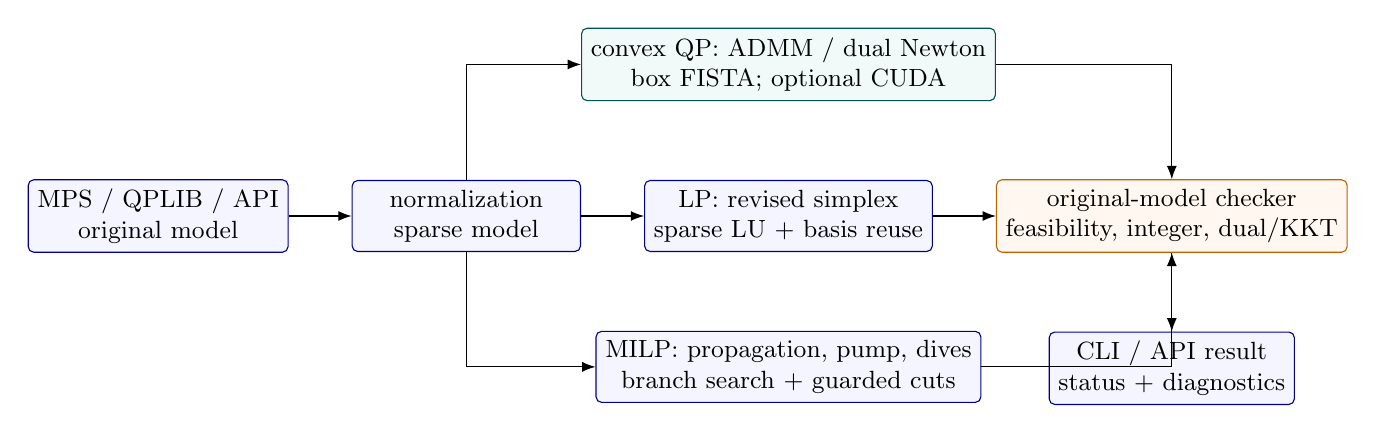
\begin{tikzpicture}[>=Latex, node distance=10mm and 8mm, font=\small,
  box/.style={draw=blue!55!black,rounded corners=2pt,fill=blue!4,align=center,minimum height=9mm,minimum width=29mm},
  gate/.style={draw=teal!65!black,rounded corners=2pt,fill=teal!5,align=center,minimum height=9mm,minimum width=31mm},
  check/.style={draw=orange!75!black,rounded corners=2pt,fill=orange!6,align=center,minimum height=9mm,minimum width=36mm}]
\node[box] (input) {MPS / QPLIB / API\\ original model};
\node[box,right=of input] (norm) {normalization\\ sparse model};
\node[box,right=of norm] (lp) {LP: revised simplex\\ sparse LU + basis reuse};
\node[box,below=of lp] (mip) {MILP: propagation, pump, dives\\ branch search + guarded cuts};
\node[gate,above=of lp] (qp) {convex QP: ADMM / dual Newton\\ box FISTA; optional CUDA};
\node[check,right=8mm of lp] (verify) {original-model checker\\ feasibility, integer, dual/KKT};
\node[box,below=of verify] (status) {CLI / API result\\ status + diagnostics};
\draw[->] (input)--(norm);
\draw[->] (norm)--(lp);
\draw[->] (norm)|-(mip);
\draw[->] (norm)|-(qp);
\draw[->] (lp)--(verify);
\draw[->] (mip)-|(verify);
\draw[->] (qp)-|(verify);
\draw[->] (verify)--(status);
\end{tikzpicture}
\caption{Functional architecture. The original problem is retained for acceptance checks alongside the normalized working model. Reference solvers run outside this core in the evaluation harness.}
\label{fig:architecture}
\end{figure*}

\subsection{Sparse LP and Basis Management}

The LP path uses sparse revised primal simplex and a bounded-variable dual simplex path. Its own sparse LU employs threshold row pivoting, fill accounting, and eta updates with periodic refactorization. No explicit dense inverse is required for the primary path. Warm starts check reduced costs and dual feasibility and fall back to a cold solve when those guards fail. A dense two-phase method remains a small-problem recovery path, and its output is still checked on the original model \cite{arch,bounded}. These choices address three common failure modes: basis singularity, excessive refactorization expense, and invalid reuse after bound or row changes.

Numerical robustness is more than a small objective difference. At a candidate $x$, an original-model row violation can be written as
\begin{equation}
 r_i(x)=\max\{\ell_i-(Ax)_i,\;0,\;(Ax)_i-u_i\}.
\end{equation}
We distinguish absolute $\max_i r_i$ from a scale-aware residual divided by a row/bound magnitude. The distinction matters for very large coefficients: a small relative residual may correspond to an unacceptable physical-unit violation. When an LP basis is numerically weak, a selective two-pass ratio test can favor a stronger pivot within the existing feasibility allowance. On one selected 16-LP public cohort, this opt-in safeguard completed and independently checked all 16, whereas retained default controls still failed on the \texttt{bandm} standard form; the test is not a random, all-Netlib success rate \cite{lpstable}.

\subsection{MILP Search and Primal Discovery}

The MILP path includes bound propagation, best-bound search with depth tie breaking, sparse LP relaxations, a root $\ell_1$ feasibility pump, and two diving heuristics \cite{arch}. The pump alternates rounding with sparse LP distance projection, applies controlled perturbations on cycles, and shares a bounded heuristic time budget. It may discover a candidate, but its distance objective does not become a valid lower bound for the original MILP. Nearly integral candidates undergo fixed-integer repair on the original model. A tree bound depends on valid relaxation processing; an incumbent depends on a separate original-model check.

Cuts illustrate the tension between mathematical strength and computational usefulness. Binary cover and opt-in lifted-cover cuts can strengthen a relaxation within their validity domain. A Gomory-style tableau separator improved root bounds in an earlier small development experiment, but the later end-to-end paired evaluation showed a negative search effect, detailed in Section~\ref{sec:results}. The recommended profile therefore omits that optional cut flag; the implementation remains available as an experiment \cite{iter37}. General branch-and-bound status relies on numerical safety margins and is not an exact-rational proof. A separate, strict small-binary integer-data mode offers checked enumeration and witness verification for its declared subset only \cite{arch}.

\subsection{Convex QP and Selective GPU Use}

For continuous convex QP, the project implements sparse scaled ADMM with Jacobi-preconditioned conjugate gradients and polishing, a magnitude-scaled dual Newton/CG specialist for positive diagonal Hessians with equality rows, and accelerated projected gradient for box QP \cite{arch,qp9002}. The form-specific method choice is substantive: a million-dimensional sparse box problem does not require the same linear system treatment as a constrained QP with many equality rows.

The optional CUDA path keeps sparse CSR data resident and executes double-precision FISTA kernels for the box-QP class. It should be assessed by end-to-end time including transfers and setup, not only kernel time. Unsupported CUDA selections fail explicitly, and CPU-only builds do not masquerade as GPU runs \cite{arch,gpu03}. Literature reports GPU optimization gains under suitable structure \cite{gpuadmm2020,cupdlp2025}; those results are context, not evidence of this project's speed.

\section{Algorithmic Invariants and Numerical Mechanisms}

The broad architectural labels above hide the practical contract required at each boundary. The project does not have a single oracle that can solve every recognized input. It has multiple numerical paths with eligibility checks, deadlines, fallbacks, and a common final acceptance layer. The following details make the claimed from-foundations implementation and its limits more inspectable.

\subsection{Bounded-Variable Dual Simplex at Tree Nodes}

The bounded LP engine represents each ranged row by a logical variable $r_i$ and equality $Ax-r=0$, while retaining native lower and upper bounds on both $x$ and $r$ \cite{bounded}. When a branch changes a variable bound, the matrix structure need not be reconstructed with an extra inequality row; basis statuses can be reused. The dual phase uses a sparse basis factorization, row-wise pivot computation, bound-flipping ratio logic, and steepest-edge-inspired pricing. Products of eta updates are periodically refactored. Cost shifts and temporary artificial bounds are cleanup devices, not final proof data: they must be removed before original-objective acceptance. The older sparse engine remains a fallback if the bounded path cannot validate a result.

For a candidate node lower bound $\beta$, the crucial invariant is $\beta\leq z^*_{\rm node}$ in minimization sense, within the declared numerical safety policy. A node can only be pruned against an incumbent $z^{\rm inc}$ if a valid lower bound satisfies $\beta\geq z^{\rm inc}$ after margins. The implementation recomputes a Lagrangian bound on original rows in extended precision before cutoff, using a guard of $200\tau(1+|z^{\rm inc}|)$ for configured tolerance $\tau$ in its documented policy \cite{bounded}. This makes a false strong bound more expensive to publish than a missing bound. It does not turn the floating-point search into an exact mathematical proof.

An LP infeasibility return also needs more than failure to find a point. The bounded path normalizes a final BTRAN/Farkas multiplier and checks an interval implied by original variable and row bounds; a ray relying on artificial bounds or fragile infinite-bound arithmetic is declined \cite{bounded}. Other outcomes---iteration cap, rejected certificate, numerical error, or time limit---remain separate statuses. This distinction is necessary in a MILP tree, where an invalid infeasibility claim could prune an entire feasible branch.

\subsection{Primal Heuristics Are Not Lower-Bound Engines}

The feasibility pump and dives spend time to discover incumbents, while the LP relaxation supplies potential bounds. This separation is a mathematical invariant. Let $\hat x$ be an integer-rounded target and consider a pump projection that minimizes an $\ell_1$ distance to $\hat x$ under relaxed original rows. Its objective is \emph{distance}, not $c^\top x$ from Eq.~\eqref{eq:lp}; even an optimal distance projection says nothing directly about the MILP objective lower bound. A rounded point must satisfy every original row and integer restriction before it becomes an incumbent. The root pump is limited to a small share of the global budget and restores the validated pre-heuristic state when an unfinished cut LP or projection cannot be trusted \cite{arch}. Bounded runtime and original-model repair are as important as the rounding formula on a difficult search.

The same logic applies to optional cuts. A valid inequality may strengthen $z_{\rm LP}$, but obtaining it can require tableau work, new rows, a basis transition, and later refactorization. The relevant engineering objective is not simply $\Delta z_{\rm root}$; it is the resulting distribution of validated incumbents, proofs, node throughput, memory, and numerical fallbacks under a fixed wall-clock budget. The 60-instance ablation is a direct example. The project retains an opt-in separator for investigation while declining to recommend it as a default after its measured end-to-end regression \cite{iter37}.

\subsection{A Structure-Specific QP Dual Bound}

For a strictly positive diagonal Hessian $H={\rm diag}(h_j)$ and finite equality rows $Ax=b$, the specialist first whitens curvature and scales row magnitudes, then reconstructs primal and dual variables in original units \cite{diagmethod}. For an original-space multiplier $y$, the bound-constrained Lagrangian minimization separates by coordinate. With $d=c+A^\top y$ and box bounds $L_j\leq x_j\leq U_j$, its minimizer is
\begin{equation}
 w_j(y)=\operatorname{clip}\!\left(-d_j/h_j,L_j,U_j\right).
 \label{eq:clip}
\end{equation}
Substitution gives a computable numerical dual lower bound
\begin{equation}
 D(y)=-b^\top y+\sum_j\left[\tfrac12h_jw_j^2+d_jw_j\right]+c_0,
 \label{eq:qpdual}
\end{equation}
where $c_0$ is the model offset. For ranged rows, the relevant row endpoint depends on the sign of the multiplier; the implementation's documented formula handles that generalization \cite{diagmethod}. This certificate is stronger than trusting a small projected gradient alone when $h_j$ is tiny. It is valid for the declared strictly positive diagonal structure and numerical arithmetic, not a generic duality proof for arbitrary indefinite $Q$.

Scaling is part of correctness, not only speed. If $x=sDz$, with $D_{jj}=h_j^{-1/2}$ and row normalization $E$, the matching multiplier reconstruction is $y_{\rm original}=sE\,y_{\rm scaled}$ \cite{diagmethod}. Recovering $x$ but forgetting to transform $y$ would corrupt original-model stationarity and any dual bound. The original QPLIB 9002 case has diagonal entries spanning many orders of magnitude and bounds around $10^{11}$; it therefore exercises exactly this risk.

\subsection{Narrow Exact Mode versus General Numerical Search}

The optional small-binary proof path is qualitatively different from numerical branch-and-bound. It accepts at most 36 movable binaries, 32 rows, and 128 original columns under strict integer-data and structure guards; it uses checked 64-bit arithmetic with magnitude limits and split enumeration \cite{binaryproof}. Completion of all required work can prove an optimum or infeasibility for that restricted class. Unsupported rows, nonintegral source literals, arithmetic overflow risk, or exhausted work cannot be promoted into proof metadata. A separately written checker rereads source decimal text with exact fractions and recomputes the witness/absence test. This is useful for a narrow public example but cannot be extrapolated to general MILP, much less industrial-scale MILP.

The resulting public interface should expose \emph{what} made a claim: numerical root/bound search, a checked feasible point, or the strict exact path. Without such metadata, the word optimal encourages a reader to infer more than the evidence supports. Conversely, an explicit numerical-error status is a useful outcome when the alternative is an unsound point.

\section{Validation and Claim Semantics}

\subsection{A Hierarchy of Evidence}

Optimization status words encode different strengths of assertion. A feasible MILP vector checked against the original file is an incumbent, not an optimal solution. A finite search bound with a small relative gap is a numerical stopping criterion, not exact arithmetic. A general LP or QP status relies on feasibility, duality, and KKT tolerances; an exact small-binary certificate applies only to an explicitly guarded subset \cite{arch}. Incorrect branch-and-bound decisions can arise from floating-point numerics, which motivates independent checking and conservative status language \cite{hoen2025,refine2016}.

For every reported MILP vector in the historical benchmark, a separate HiGHS 1.12.0 reader checked integrality and original-model feasibility and compared the objective with the published MIPLIB solution file. The reference value was not supplied to the search engine. This validates a returned point under declared tolerances and checks agreement of seven reported numerical optima with published values; it is not a proof that every difficult model is solved \cite{mip240}. The MIPLIB best-known file used by that experiment was \smallpath{miplib2017-v32.solu}; the MIPLIB site now lists a later version, so current best-known data must not silently replace the frozen experiment's reference \cite{miplibdownload}.

For a convex QP, representative acceptance quantities include primal row/bound residual, projected stationarity, complementarity, and a dual lower bound when valid. For positive diagonal $Q$, minimizing each separable Lagrangian coordinate can provide a numerical dual bound. The returned primal-dual gap must be interpreted with the same original model, objective sense, and scaling. A converged iterate is not a universal bound on objective error if curvature is tiny or an applicable lower bound cannot be formed \cite{qp9002,arch}.

\subsection{Reproducibility Units}

The correct unit of comparison is the tuple (source/binary hash, option profile, input/reference version, budget, machine, independent checker). The 240-instance experiment used a frozen engine SHA-256 beginning \texttt{e40e849f69d2}, MIPLIB benchmark list \smallpath{benchmark-v2.test}, solution file v32, 300 seconds per instance, a 100-million-node cap, and a requested gap of $10^{-6}$. Five Kaggle CPU sessions covered all 240 rows; one platform cancellation left 44 of 60 records in a batch, which were recovered and included. A consolidator rejected duplicate or missing instance records \cite{mip240}. These specifics matter because a later algorithm revision is a different treatment.

The paired 60-instance cut study used one frozen executable (hash beginning \texttt{e379b12cb513}), the same host, the same 300-second cap, and a single option difference \cite{iter37}. The GPU study used a Tesla T4 with 15,360 MiB device memory, four host CPU cores, and three repeats for each of 15 size/backend combinations \cite{gpu03}. Cloud contention and three repeats limit statistical inference. A later merge-verification report records matching fixed-work tests but also wall-clock heuristic nondeterminism and the inability to rebuild a frozen earlier executable byte-identically on the local machine; the study therefore identifies source and measured-binary provenance separately \cite{merge}.

\begin{table*}[t]
\centering\small
\caption{Evidence cohorts are intentionally separate. Counts cannot be pooled into a single current-engine score.}
\label{tab:cohorts}
\begin{tabularx}{\textwidth}{@{}p{0.17\textwidth}p{0.16\textwidth}p{0.23\textwidth}X@{}}
\toprule
Cohort & Scale and budget & What it supports & What it does not support\\
\midrule
Historical complete MIPLIB 2017 & 240 public MILPs; 300 s each; Kaggle shared CPU & Complete outcome and independent-point ledger for one frozen engine & Performance of later fixes, current-profile 240 score, or fair cross-solver wall-time ranking\\
Cut ablation & 60 public MILPs; 300 s; same binary/host & Paired effect of one optional cut flag on this slice & General proof that cuts never help; full 240-instance corrected-profile outcome\\
Stable LP ratio test & 16 selected public LPs; opt-in flag & Completion and original-model checks on selected path & Default robustness on all Netlib / industrial LPs\\
QPLIB 9002 specialist & One hard original public QP, repeated local CPU & Original-model relative KKT/dual-gap success with an absolute-violation caveat & A successful OSQP head-to-head comparison or general constrained-QP scalability\\
T4 box-QP study & Planted sparse family, $10^4$--$10^6$ variables, 3 repeats/backend & Equal-contract CPU/GPU crossover on one family/device & GPU LP/MILP performance or production workload latency distribution\\
\bottomrule
\end{tabularx}
\end{table*}

\section{Evaluation Design: What a Comparison Must Hold Fixed}

\subsection{Population, Versions, and Denominators}

A benchmark numerator without a declared denominator is especially misleading in MILP. A development-cohort tally of useful outcomes---which may include checked feasible points and corroborated infeasible statuses---answers a different question from complete coverage on 240 MIPLIB benchmark models. The former may guide engineering; the latter audits generality on a recognized hard public set. We keep the complete historical cohort, later 60-model public slice, selected LP/QP cases, and synthetic GPU generator distinct in Table~\ref{tab:cohorts}. None is converted into a single pooled success percentage. MIPLIB 2017 names a fixed benchmark set, whereas its best-known solution/status files evolve; the historical run used solution file v32, not the newer file visible in September 2026 \cite{mip240,miplibdownload}. A reproducible rerun should archive the exact instance and reference bytes with hashes, not only the benchmark name.

The denominator for validated feasible points includes both optimal and nonoptimal incumbents. In the 240-instance outcome ledger, 69 valid points means seven numerical-optimum points plus 62 other feasible points. The independently corroborated infeasible case is not a feasible point. The 170 no-point cases are not all proven infeasible; they are unresolved within the declared budget. Reporting these as four mutually exclusive classes makes the arithmetic transparent. A useful next study should also stratify by binary/general-integer structure, matrix density, row/column scale ratio, root relaxation status, and incumbent gap, rather than publishing only one aggregate.

\subsection{Accuracy Before Speed}

The primary acceptance key should be objective and constraint agreement at a specified tolerance, followed by elapsed time on the same task. Two solvers returning different qualities cannot be fairly compared by time alone. For LP, a result table should include primal and dual residuals, objective gap, and status. For MILP, it should distinguish time to first \emph{independently valid} point, best objective, best valid bound, relative gap, and time to a numerical optimum under matching criteria. For QP, KKT residuals and any applicable dual bound should accompany time. If a solver times out, the observation is censored at the budget; replacing it with an invented completion time biases performance profiles \cite{dolanmore2002}.

More generally, competition scoring may combine runtime, accuracy, memory, robustness, and domain fit. Without the organizer's exact rubric and raw test rows, an aggregate score cannot identify which component improved or remains deficient. This paper therefore states concrete project measurements and their units, while treating any final competition score as unknown.

\subsection{Paired Ablations and Holdouts}

Ablation is strongest when a single option changes while executable, input order, budget, hardware, and checker remain fixed. Iteration 37 approached that standard by pairing cut-on and cut-off on the same 60 public models with one frozen binary \cite{iter37}. Even then, shared CPU load and heuristic timing variation can change incumbents. Repeating order-swapped runs and reporting per-instance differences would narrow uncertainty. By contrast, comparing a recent run on one machine with an old historical run on another cannot isolate an algorithm change. This is why the cut study is presented separately from the 240 full ledger.

Development and holdout sets play different roles. The bounded dual simplex iteration recorded both development and fresh holdout effects, including a five-versus-one completion contrast at 30 seconds on a 15-model holdout \cite{iter30}. The memory-trail iteration recorded a favorable selected mechanism measure and a less favorable ten-model search holdout \cite{iter33}. Such reversals are informative: tuning against a particular micro-metric may move cost elsewhere in the pipeline. Future profile promotion should require prespecified, end-to-end public holdout criteria that include regressions, not only root-bound strength or allocation savings.

\subsection{Resource and Energy Measurement}

Wall time is not CPU time; CPU time is not energy; and GPU kernel timing is not full-process latency. The T4 measurements include setup and transfers but were made in a shared cloud session, with no isolated power meter or controlled board-power sampling \cite{gpu03}. A future energy-per-validated-solve experiment should log start/end timestamps, device and CPU power sampling, idle baseline, successful output checks, and repeated matched workloads. A consistent metric might be joules per validated solution at a fixed tolerance, with total energy reported separately for failures/timeouts. Until such a protocol is executed, no solver energy-efficiency percentage belongs in the SIH26119 results.

\section{Public-Benchmark Results}\label{sec:results}

\subsection{Complete Historical MIPLIB 2017 Ledger}

Figure~\ref{fig:mip240} visualizes the outcomes of all 240 MIPLIB 2017 benchmark instances on the frozen historical engine. Seven instances returned solver-reported numerical optimality statuses matching the published objective; one was reported infeasible in agreement with the published status. Of the 69 instances with checked feasible points, 62 had no optimality conclusion. A further 170 instances produced no feasible point at the time limit. There were zero vectors rejected by the independent checker and zero reported-answer disagreements with the published solution file \cite{mip240}. The seven are not evidence of a fully general exact proof engine; the separately restricted binary proof mode is not being substituted for them.

\begin{figure}[t]
\centering
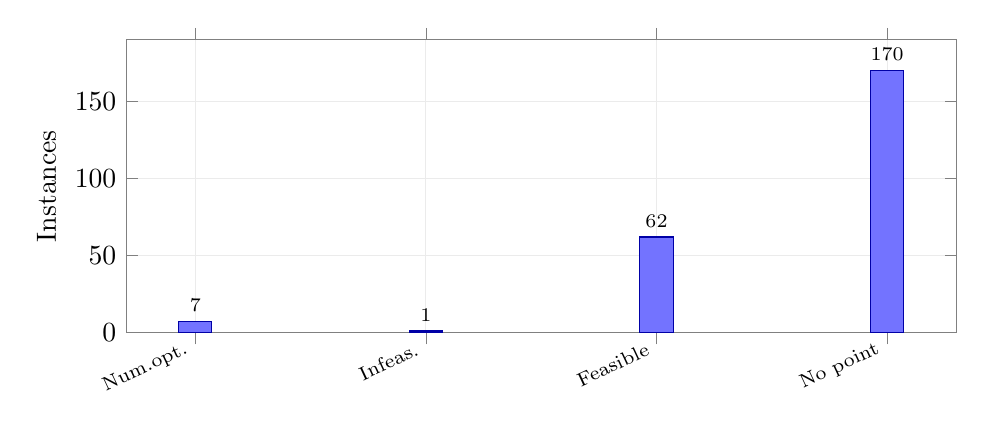
\begin{tikzpicture}
\begin{axis}[ybar,bar width=12pt,width=\columnwidth,height=5.3cm,
  ymin=0,ymax=190, ylabel={Instances},
  symbolic x coords={Num.opt.,Infeas.,Feasible,No point},xtick=data,
  x tick label style={rotate=25,anchor=east,font=\scriptsize},
  nodes near coords,nodes near coords style={font=\scriptsize},
  axis line style={black!50},tick style={black!50},grid=major,grid style={black!8}]
\addplot[fill=blue!55,draw=blue!65!black] coordinates {(Num.opt.,7) (Infeas.,1) (Feasible,62) (No point,170)};
\end{axis}
\end{tikzpicture}
\caption{Mutually exclusive statuses for all 240 historical MIPLIB 2017 results. ``Feasible'' means a checked point without numerical optimality status; ``no point'' is unresolved, not an infeasibility claim.}
\label{fig:mip240}
\end{figure}

The seven matched objective values occur on \texttt{eil33-2}, \texttt{app1-1}, \texttt{decomp2}, \texttt{hypothyroid-k1}, \texttt{markshare\_4\_0}, \texttt{neos8}, and \texttt{rmatr100-p10}. The one reported infeasibility is \texttt{neos859080} \cite{mip240}. The result is meaningful as a complete, independently audited outcome ledger, but eight status conclusions out of 240 are far below the coverage needed to characterize this as a general hard-MILP solution. The 170 unresolved cases should remain visible in a PPT or submission summary rather than be hidden behind a subset of wins.

The historical report also flags 31 open-node memory-guard stops, 27 unresolved root LPs under its iteration cap, and two factorization-resource exits \cite{mip240}. Its diagnostic table is not a disjoint partition of the four plotted outcomes and should not be summed into a second total. Later iterations separately targeted memory retention and root LP handling; they cannot be treated as if they changed the 240 historical observations. The current corrected profile has not been rerun and consolidated on all 240 instances in the local evidence set.

\subsection{End-to-End Cut Ablation on 60 Instances}

Table~\ref{tab:ablation} gives the paired 60-instance comparison. Earlier root-bound experiments made Gomory cuts look promising, but activating them at a 300-second search budget yielded two numerical optima and 19 checked points, versus three and 21 with the flag absent. Nodes processed fell from 7.75 million to 5.95 million, and bounded-engine fallback/cold-start counts rose sharply \cite{iter37}. A cut can be valid and locally improve an LP bound while harming wall-clock search if extra rows disrupt warm starts or inflate per-node cost. On \texttt{decomp2}, disabling the flag produced a root numerical optimum in one node, whereas enabling it processed 8,930 nodes without a final point; \texttt{csched008} is a counterexample that benefited from the cut flag. The decision is profile-specific, not a theorem that Gomory cuts are bad.

\begin{table}[t]
\centering\small
\caption{Same-binary 60-instance Gomory-cut ablation, 300 seconds per instance \cite{iter37}.}
\label{tab:ablation}
\begin{tabular}{@{}lrr@{}}
\toprule
Metric & Cuts on & Cuts off\\
\midrule
Numerical optima & 2 & \textbf{3}\\
Checked feasible points & 19 & \textbf{21}\\
Roots solved & 49 & 49\\
Nodes explored & 5,947,089 & \textbf{7,753,820}\\
Bounded-engine fallbacks & 1,984 & \textbf{305}\\
Cold starts & 2,030 & \textbf{282}\\
Unresolved nodes & 20 & \textbf{9}\\
Rejected points / disagreements & 0 / 0 & 0 / 0\\
\bottomrule
\end{tabular}
\end{table}

Separate iteration-30 experiments showed that bounded dual simplex increased development completion \emph{run records} from 17/54 to 23/54 (27 models, two repeats each) at 30 seconds, fresh 15-model holdout completions from one to five, and selected public LP completions from 15/16 to 16/16 under their particular profiles \cite{iter30}. These are valuable mechanism tests, not independent evidence that the final 240-instance coverage rose by the same fraction. In iteration 33, shared bound trails reduced fixed-node memory by 1.44--9.39$\times$ on six selected models, but a ten-model holdout explored fewer nodes \cite{iter33}. Both benefit and regression must be carried forward to a full rerun.

\subsection{QP Numerical Results and Their Limit}

The original QPLIB 9002 case has 2,890 variables, 1,649 equality rows, and 9,690 linear nonzeros. A structure-specific, magnitude-scaled diagonal-Hessian solver produced a median 4.2754-second local CPU completion across three repeats. Independent original-model checks gave relative primal feasibility $8.57\times10^{-8}$, projected stationarity $2.41\times10^{-16}$, relative complementarity $4.12\times10^{-11}$, and a relative primal/dual gap $7.85\times10^{-11}$ \cite{qp9002}. Yet the maximum \emph{absolute} constraint violation was 2.381 in model units. The relative certificate therefore does not automatically establish suitability for an application with an absolute tolerance below that value.

Three selected public QPLIB models passed independent original-model KKT checks, but only two of three completed the unchanged reference-solver comparison: the OSQP 1.0.5 run on original 9002 timed out under the retained protocol. No finite speedup-to-solution over OSQP can be computed from that timeout \cite{qp9002}. A QPLIB LP export also changed Hessian entries relative to the original QP, which is why original-file checking matters. This experiment is evidence for a difficult \emph{specific structure}, not for arbitrary constrained or nonconvex QP.

\subsection{Repeated GPU Crossover on Box QP}

Figure~\ref{fig:gpu} and Table~\ref{tab:gpu} use end-to-end measurements from one planted sparse tridiagonal box-QP family. The same accuracy contract was applied to one CPU thread, four CPU threads, and the T4 GPU; all 45 runs (five sizes, three backends, three repeats) returned an accepted optimum under the generator check. Worst relative objective error was $8.2\times10^{-14}$ and worst maximum solution error was $6.0\times10^{-6}$, below the declared $10^{-4}$ threshold \cite{gpu03}. The GPU is slower at 10,000 variables, approximately crosses a single CPU thread near 50,000, and outperforms four CPU threads by 2.38$\times$ at one million. These ratios include setup/transfers and are not applicable to a general MILP or linearly constrained QP.

\begin{figure}[t]
\centering
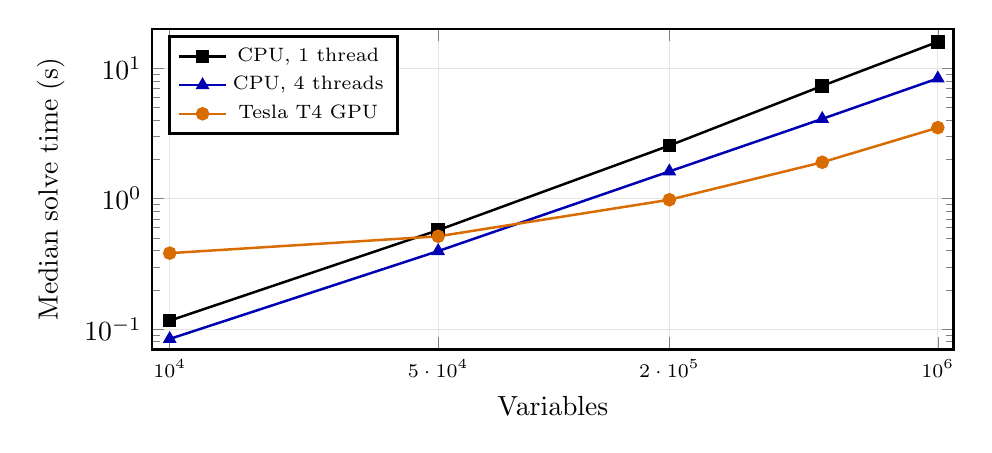
\begin{tikzpicture}
\begin{loglogaxis}[width=0.97\columnwidth,height=5.65cm,
  xmin=9000,xmax=1100000,ymin=0.07,ymax=20,
  xlabel={Variables},ylabel={Median solve time (s)},
  xtick={10000,50000,200000,1000000},
  xticklabels={$10^4$,$5\cdot10^4$,$2\cdot10^5$,$10^6$},
  x tick label style={font=\scriptsize},
  legend style={font=\scriptsize,at={(0.02,0.98)},anchor=north west},
  grid=major,grid style={black!10},
  line width=0.9pt,mark size=2pt]
\addplot[color=black,mark=square*] coordinates {(10000,.116) (50000,.573) (200000,2.551) (500000,7.314) (1000000,15.923)};
\addlegendentry{CPU, 1 thread}
\addplot[color=blue!70!black,mark=triangle*] coordinates {(10000,.084) (50000,.396) (200000,1.616) (500000,4.086) (1000000,8.342)};
\addlegendentry{CPU, 4 threads}
\addplot[color=orange!85!black,mark=*] coordinates {(10000,.382) (50000,.514) (200000,.980) (500000,1.900) (1000000,3.501)};
\addlegendentry{Tesla T4 GPU}
\end{loglogaxis}
\end{tikzpicture}
\caption{Median of three end-to-end runs per backend and size on one planted box-QP family \cite{gpu03}. This is a crossover experiment, not a universal solver ranking.}
\label{fig:gpu}
\end{figure}

\begin{table}[t]
\centering\small
\caption{Repeated box-QP medians in seconds; all three repeats per cell passed the same generator accuracy check \cite{gpu03}.}
\label{tab:gpu}
\begin{tabular}{@{}rrrr@{}}
\toprule
$n$ & CPU 1 & CPU 4 & T4 GPU\\
\midrule
10,000 & 0.116 & \textbf{0.084} & 0.382\\
50,000 & 0.573 & \textbf{0.396} & 0.514\\
200,000 & 2.551 & 1.616 & \textbf{0.980}\\
500,000 & 7.314 & 4.086 & \textbf{1.900}\\
1,000,000 & 15.923 & 8.342 & \textbf{3.501}\\
\bottomrule
\end{tabular}
\end{table}

\section{Failure-Mode Studies on Hard MILPs}

The complete MIPLIB ledger is a baseline; the later iteration reports are mechanism studies. Their value is not that every local change increased the number of solved models. Rather, each isolates a reason that a large search can stall or misreport a result. Figure~\ref{fig:memory} and Table~\ref{tab:mechanisms} assemble four examples without combining them into an invented current-engine benchmark score.

\subsection{Frontier Memory: Sharing Bounds across Siblings}

Before iteration 33, every queued tree node retained complete lower- and upper-bound vectors. With $F$ open nodes and $n$ variables, this has an $O(Fn)$ storage component even when each branch modifies only one or two bounds. The replacement stores a pointer to a shared ancestry of bound changes; descendants share their parents' records. On pop, bounds are reconstructed by walking the trail and applying monotone max/min tightenings \cite{iter33}. The method trades cheaper node storage for reconstruction work, so it is not automatically faster.

Figure~\ref{fig:memory} shows measured memory on six selected models. The reduction ranges from 1.44$\times$ for the 30-column \texttt{gen-ip054} to 9.39$\times$ for the 2,985-column \texttt{lotsize}; the reported old/new values are process measurements, not bytes attributable exclusively to nodes \cite{iter33}. Four models reached the same 120,000-node cap in both builds. \texttt{swath} and \texttt{lotsize} hit time limits, so their old and new bars do not represent identical node counts. That qualification matters more than a visually impressive ratio.

\begin{figure*}[t]
\centering
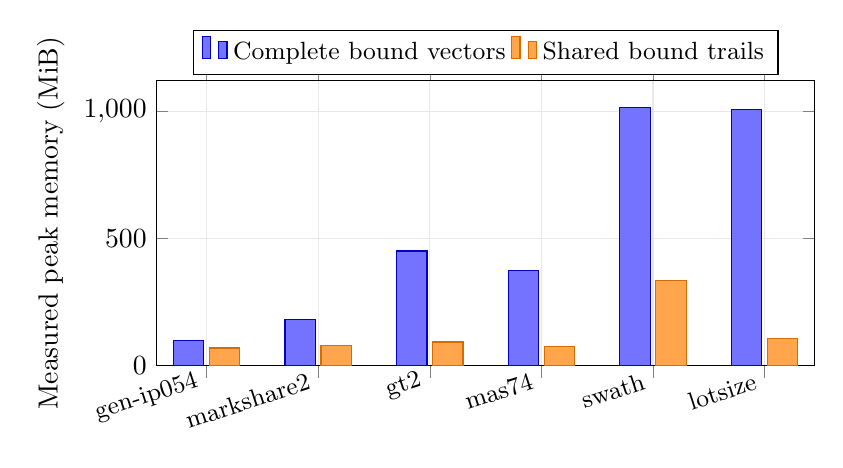
\begin{tikzpicture}
\begin{axis}[ybar,bar width=11pt,width=0.82\textwidth,height=5.2cm,
  ymin=0,ymax=1120,ylabel={Measured peak memory (MiB)},
  symbolic x coords={gen-ip054,markshare2,gt2,mas74,swath,lotsize},
  xtick=data,x tick label style={font=\small,rotate=18,anchor=east},
  legend style={font=\small,at={(0.5,1.02)},anchor=south,legend columns=2},
  grid=major,grid style={black!9},enlarge x limits=0.09]
\addplot[fill=blue!55,draw=blue!75!black] coordinates
  {(gen-ip054,100.8) (markshare2,182.1) (gt2,451.0) (mas74,375.2) (swath,1013.4) (lotsize,1008.9)};
\addplot[fill=orange!70,draw=orange!85!black] coordinates
  {(gen-ip054,69.9) (markshare2,80.3) (gt2,93.4) (mas74,76.8) (swath,336.4) (lotsize,107.5)};
\legend{Complete bound vectors,Shared bound trails}
\end{axis}
\end{tikzpicture}
\caption{Iteration-33 memory mechanism experiment \cite{iter33}. The first four pairs used equal node counts; the last two were time-limited and explored different numbers of nodes. Lower memory does not by itself establish a higher completion rate.}
\label{fig:memory}
\end{figure*}

The correctness issue in this representation is subtle. Domain propagation can derive bounds beyond the explicit branch decision, and the implementation stops propagation after ten passes rather than at a mathematical fixed point. If a child inherits only branch bounds, it may re-derive a different set and alter the search. An initial per-node memoization cap did just that on \texttt{binkar10\_1}; bound tightenings jumped from 26,618 to 6,457,700 and eight of 32 fixed-work checks differed. The retained implementation memoizes root/ancestor propagated changes onto shared trails and passed 32 of 32 fixed-work equivalence comparisons, with zero status, objective, bound, node, LP-iteration, or tightening mismatches \cite{iter33}. This is a useful example of why a memory optimization needs a semantic gate, not merely a memory chart.

The measured search trade-off is also nonuniform. Development runs processed about 19.8\% more nodes per second under the new representation; a fresh ten-model public holdout processed 40,621 nodes versus 47,947 for the control. Deep paths through wide models cost more to materialize. A separate 17-instance memory-guard rerun cut guard stops from 16 to one and improved checked incumbents on ten instances, worsened one, but produced no new proof at 300 seconds \cite{iter33}. Thus the change buys headroom and some point quality, not a documented universal throughput or proof gain.

\subsection{Root-LP Budget Is Different from Node-LP Budget}

Iteration 34 diagnosed a second avoidable stop. Twelve selected difficult roots all halted at exactly 10,000 simplex iterations, the same cap used for warm node LPs. A cold root can need more iterations than a small bound-change child. The opt-in root-specific allowance raises only the root and root cut-round cap; it leaves node and heuristic budgets unchanged \cite{iter34}. On the 12 diagnosed instances, root completions changed from zero to eight and one instance, \texttt{neos-827175}, returned a numerical optimum matching its published objective. On a prespecified five-model root-stuck holdout, root completions changed from zero to three, but none yielded a final solution. Across both sets, 11 previously stuck roots finished, yet only one resulted in a checked point. This separates a necessary prerequisite (the root LP finishes) from the desired outcome (a useful integer point or proof).

For the remaining roots, lifting the cap exposed the actual throughput problem: models with thousands of rows ran at only tens or a few hundreds of pivots per second and still exhausted 300 seconds. For several newly solved roots, search then had little time left or descendants began from a cold basis. A higher cap should therefore be framed as resource allocation, not an algorithmic speedup. A future study should report root time, root bound quality, and integer-search time in separate columns rather than replacing a no-root failure with a solved count.

\subsection{Basis Continuity through Optional Cut Removal}

The next study addressed a cold-start side effect. When slack tableau cuts were removed after the root, the older implementation discarded the entire LP basis. But each removed row had its own basic logical column and zero dual; deleting that row together with its basic logical can preserve the basis structure, subject to the existing warm-start verification \cite{iter35}. On six mechanism instances at 300 seconds, aggregate nodes rose from 16 to 6,618 and cold starts fell from 21 to seven. On seven fresh point-producing instances, cold starts fell from 37 to eight while validated-point count remained six on each side.

This was not an unqualified success. The prespecified aggregate unresolved-node criterion failed: six unresolved nodes in the control became seven in the candidate, because some searches ran hundreds of times farther and met different downstream numerical problems. The post hoc normalized failure rate improved, but a rate was not the preregistered criterion; the report explicitly preserves that deviation \cite{iter35}. This is a valuable negative-control lesson. When an intervention greatly changes exposure (nodes visited), both absolute failure count and failures per thousand nodes should be declared in advance. A favorable denominator discovered after the run should not erase an adverse prespecified result.

\subsection{Resource-Limit Recovery without Claim Inflation}

Iteration 36 then caught a factorization-fill resource exception occurring in a cut-strengthened relaxation. Previously this could terminate the entire solve as if the input were invalid. The revised path returns a failed relaxation; if optional separator rows are present, it discards them and retries the node once \cite{iter36}. On \texttt{neos8}, 91 separator rows were discarded; the model moved from an abort to a reported zero-gap numerical optimum at objective $-3719$ in 83 seconds and 67 nodes, matching the published value. Two other large mechanism cases still produced no solved root. On the eight largest fresh public instances, control and candidate were identical: no root solved at 300 seconds. The gain is reliable failure handling and one recovered numerical optimum, not general large-model scalability.

\begin{table*}[t]
\centering\small
\caption{Distinct mechanism experiments, each against its own declared control. They are not additive gains on one 240-instance final run.}
\label{tab:mechanisms}
\begin{tabularx}{\textwidth}{@{}p{0.16\textwidth}p{0.23\textwidth}p{0.28\textwidth}X@{}}
\toprule
Mechanism & Comparison cohort & Positive observation & Retained limitation\\
\midrule
Shared bound trails \cite{iter33} & Six selected memory tests; ten fresh search holdouts; 17 guard cases & Measured memory falls 1.44--9.39$\times$ on selected models; guard stops 16 to one on targeted rerun & Fresh holdout nodes fall 47,947 to 40,621; no new proof among guard cases\\
Root iteration allowance \cite{iter34} & Twelve diagnosed and five fresh root-stuck models & Root completion 0 to 8 and 0 to 3; one matched numerical optimum & Ten of 11 newly completed roots still do not yield a final checked point\\
Basis retention after cut purge \cite{iter35} & Six mechanism and seven fresh point-producing models & Nodes 16 to 6,618 in mechanism set; fresh cold starts 37 to eight & Six versus seven unresolved nodes violates one declared aggregate criterion\\
Resource-limit recovery \cite{iter36} & Three known fill-limit cases; eight largest fresh models & \texttt{neos8} no longer aborts and returns $-3719$ with zero numerical gap & Two known and all eight largest fresh cases still have no solved root\\
\bottomrule
\end{tabularx}
\end{table*}

The later 60-instance cut ablation remains the integration test for these mechanisms under a realistic 300-second budget. It showed that keeping Gomory cuts enabled still cost validated answers despite these targeted fixes \cite{iter37}. The correct engineering conclusion is to keep mechanism improvements that pass their own safety gates, remove the cut flag from the recommended profile, and rerun the complete public set on the resulting frozen configuration before claiming a new overall coverage number.

\section{Verification Case Studies and Input Contracts}

A trustworthy optimization engine needs examples in which the obvious-looking shortcut is wrong. The local reports preserve several such cases. They are more informative than a list of successful unit tests because they show which claim would have been unsound without a guard.

\subsection{Near-Integer Does Not Mean Feasible}

On a retained \texttt{blend2} node, simply rounding the LP point produced an original-model absolute row violation of approximately $2.001\times10^{-6}$, above the project's $10^{-7}$ candidate threshold \cite{repairmethod}. The same integer assignment was feasible after a fixing LP adjusted its continuous variables. The scaled sparse fixing path returned a numerical error, whereas the project's dense two-phase fallback and unscaled sparse path returned objective about 8.015188; an independent fixing-model check put the dense candidate's maximum violation near $2.27\times10^{-13}$. This does not establish that all rejected rounded assignments are repairable. It establishes that an integer assignment should not be rejected solely because one scaled fixing method fails, and that a repaired candidate still needs its own original-row check.

The fallback is bounded: at most two seconds per attempt, no more than 20\% of remaining global time, and a cumulative allowance limited by the total solve budget; its dense tableau allocation guard remains active \cite{repairmethod}. This is a deliberate trade. Spending more time repairing may find a first incumbent, but it may displace branch search on a model where the repair fails. The published report therefore records both successful and rejected attempts rather than assuming a repaired candidate is always available.

\subsection{An Integer Fixing Cannot Prove a Node}

Suppose a tree LP yields an integer component $i=1.00000008$, sufficiently close to one for a typical numerical integer-tolerance test. A fixed-integer solve at $i=1$ can produce a feasible point with objective 80, while a branch at $i=2$ may have objective around one in the retained piecewise-linear counterexample \cite{repairmethod}. The fixing LP explores one assignment, not the entire parent domain. Thus its objective is an upper-bound candidate for a minimization MILP, never a replacement lower bound on all parent assignments. Pruning the node after repair would be incorrect even if the repaired point is perfectly feasible.

The project's correction retains the original node bound and branches on a remaining nonzero fractional integer component when the children strictly tighten valid integer bounds. Otherwise the unresolved bound is preserved rather than silently discarded \cite{repairmethod}. This is an instance of a general principle: heuristic work can improve an incumbent without granting proof authority. It also illustrates why a zero displayed integrality residual at rounded precision is not enough for numerical optimality. Branching, bounds, and incumbents must remain separate objects in the state machine.

\subsection{Equivalent MPS Text May Not Be Reader-Equivalent}

An artificial stress transformation exposed a parser convention difference. This project's MPS reader adds repeated objective-row entries for one variable, while the installed HiGHS 1.12.0 reader used for comparison consumed one of two equal repeated entries in the fixture \cite{mpsduplicates}. Twenty-four raw comparisons therefore reported objective disagreement. Those raw failures were retained. An independent exhaustive enumeration checked the intended additive-cost models, and a reference-only MPS representation that aggregated repeated coefficients into one explicit entry restored agreement on all 24 candidate vectors; other parsed fields were checked unchanged \cite{mpsduplicates}. The point is not that the initial disagreements were spurious and should be hidden. The point is that solver comparison requires a shared mathematical input contract.

For an interoperable MPS benchmark, a producer should emit one explicit objective coefficient per variable, or both readers' parsed objective vectors should be compared before timing. Otherwise an apparent solver-quality gap may be a model mismatch. Conversely, canonicalizing input for a reference check must be documented and proved mathematically equivalent; it cannot be used to change the candidate's constraints or import a reference answer. The source of truth should include original bytes, canonicalized bytes when used, and a field-by-field diff of objective, bounds, row matrix, and integrality.

\subsection{Repetition and Build Identity}

The merge-verification report demonstrates another trap: the recommended full profile uses wall-clock slices for heuristics. Three consecutive runs of the same frozen executable and flags changed the incumbent on \texttt{gen-ip002} and \texttt{mas74}; LP-iteration counts also varied on \texttt{misc03} \cite{merge}. Therefore a one-off before/after timing or objective difference under that profile cannot automatically be attributed to a source edit. Disabling timed heuristics and fixing a 2,000-node work budget yielded 16/16 exact field comparisons with zero mismatches for the LP safeguard merge. Those equivalence tests support a narrow statement about flag-off behavior at fixed work, not bitwise deterministic full-profile behavior.

The same report could not reproduce the prior frozen executable byte for byte from its stored source on this machine, plausibly because build path and link order affected the binary image. That does not invalidate measured frozen-binary runs, because those binaries and results are preserved and hash-bound. It does limit independent reconstruction of the exact artifact. A stronger release process should preserve source archive, compiler and linker versions, build flags, dependency hashes, binary hash, and the raw per-instance run ledger; separately it should test whether a clean rebuild yields the same functional outputs even if image bytes differ. This is practical research provenance, not merely release housekeeping.

\section{Illustrative Industrial Models and Translation Risk}

The repository includes a refinery teaching model and a synthetic six-period production lot-sizing MILP. In one refinery sulfur-limit sensitivity study, the profit proxy in \emph{model units} was 6.5884 at a 3.50 limit, 2.5756 at 3.48, and zero by 3.46; the solver agreed with an independent HiGHS reference on the tested model. A synthetic lot-sizing model reached objective 762 with matching reference result \cite{demo,industrial}. These are useful demonstrations of parametric sensitivity, discrete scheduling, and checked objective interpretation. They are not MRPL proprietary data or a measured refinery operating benefit. Converting a model-unit objective to INR or claiming refinery-wide energy savings would require calibrated plant data, a counterfactual baseline, and domain acceptance criteria.

An industrial trial should therefore have at least three stages: (1) data-governed model extraction, including units, feasibility tolerances, and confidentiality; (2) shadow-mode comparison with a trusted planning process on identical instances; and (3) bounded operational piloting with sign-off for infeasible, delayed, or numerically uncertain cases. Application-level value includes model preparation, integration, and human review, not just solve time. GPU deployment is justified only on eligible QP structure and when measured transfer/setup-inclusive time improves the whole workflow.

\subsection{Refinery-LP Lineage and Constraint Meaning}

The refinery example is a reformulation of the public GAMS MARCO teaching model, not an extract from MRPL's production planning system \cite{gamsmarco,industrial}. The source describes two crude choices, processing units, intermediate streams, blended products, capacity ceilings, and product quality specifications. In a compact schematic form, its planning logic is
\begin{align}
\max\quad & p^\top s-c^\top u-o^\top z,\\
\text{s.t.}\quad & Bz+u-W=0,\\
& Cz\leq k,\qquad \sum_i w_{ip}=s_p,\\
& \sum_i (q_i-\bar q_p)w_{ip}\leq 0.
\label{eq:blend}
\end{align}
The last row represents an upper-quality limit. Here $u$ is crude/material purchase, $z$ is processing, $W$ is stream use, $s_p$ is product sales, $w_{ip}$ is component $i$ assigned to product $p$, and $q_i$ is a component attribute. Equation~\eqref{eq:blend} is explanatory notation for the model family, not an assertion that the exact exported MPS uses these same symbol names. The quality row is linear because the sales volume equals the sum of blend components. Its validity still depends on how yields, sulfur, density, and price units are defined. A numerically feasible LP point cannot independently validate the engineering assumptions behind those coefficients.

In the project demo, the objective is written as costs minus revenue, so $-6.588421\ldots$ corresponds to a positive profit proxy of $6.588421\ldots$ in the teaching model's units. Tightening the fuel-oil sulfur upper limit from 3.50 to 3.40 reduces that proxy to zero, with the intermediate tested values shown in Figure~\ref{fig:sulfur}. Every point in the six-value sweep matched an independent HiGHS solve, and the candidate maximum original-model violation on the baseline was about $1.14\times10^{-13}$ \cite{demo}. The monotone response is directionally sensible for a tightening constraint, but it is not a causal estimate of a refinery's actual revenue loss. The historical source's monetary units are not present-day Indian rupees, and the team has not calibrated this model to a plant's crude slate, assay, throughput, and product specifications.

\begin{figure}[t]
\centering
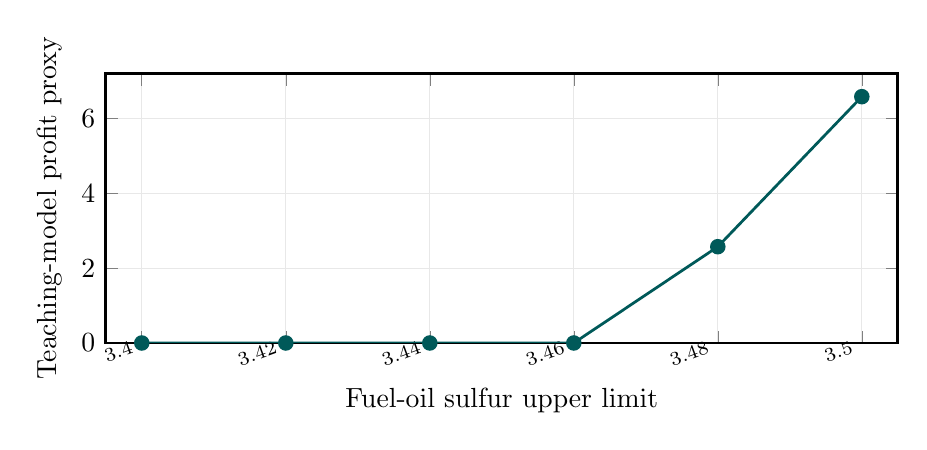
\begin{tikzpicture}
\begin{axis}[width=0.96\columnwidth,height=5.0cm,
 xmin=3.395,xmax=3.505,ymin=0,ymax=7.2,
 xlabel={Fuel-oil sulfur upper limit},
 ylabel={Teaching-model profit proxy},
 xtick={3.40,3.42,3.44,3.46,3.48,3.50},
 x tick label style={font=\scriptsize,rotate=20,anchor=east},
 grid=major,grid style={black!9},mark size=2.3pt,
 line width=1pt]
\addplot[color=teal!70!black,mark=*] coordinates
 {(3.40,0) (3.42,0) (3.44,0) (3.46,0) (3.48,2.5755621744) (3.50,6.5884214767)};
\end{axis}
\end{tikzpicture}
\caption{Six checked MARCO teaching-model sensitivity results \cite{demo}. The vertical axis is not INR or measured MRPL profit.}
\label{fig:sulfur}
\end{figure}

\subsection{Discrete Production and Transportation Cases}

The six-period production example demonstrates why LP alone is insufficient when setup decisions are indivisible. A standard lot-sizing abstraction minimizes production, inventory, and fixed setup cost:
\begin{align}
\min\quad & \sum_{t=1}^{T}\bigl(a_tq_t+h_tI_t+f_ty_t\bigr),\\
\text{s.t.}\quad & I_t=I_{t-1}+q_t-d_t,\\
& 0\leq q_t\leq K_ty_t,\\
& y_t\in\{0,1\}.
\label{eq:lotsize}
\end{align}
The binary $y_t$ activates capacity $K_t$, and the balance row links periods through inventory $I_t$. Equation~\eqref{eq:lotsize} is a schematic model template; the project-generated instance has its own six-period numerical data and final empty-stock requirement \cite{industrial}. Its verified objective of 762 is a useful functional test: the engine must parse the MILP, find an integer-feasible schedule, and agree with an independent reference on the optimum \cite{demo}. It is not evidence that a multi-plant industrial lot-sizing instance with thousands of setups will finish within a practical deadline.

The repository also builds a small transportation LP from GAMS TRNSPORT data: two plants, three demand markets, capacities, and distances \cite{gamstrnsport,industrial}. This exercises row senses, demand satisfaction, nonnegative shipment flow, and cost interpretation. Again, reference agreement on the exported model tests a solver pipeline, not whether those historical supply-chain parameters represent a present Indian logistics network. The role of such literature cases is to bridge a mathematical benchmark and a domain conversation: they supply interpretable decisions and perturbations without implying access to confidential operational data.

\subsection{Design of a Plant-Relevant Shadow Trial}

For a plant decision, a solver candidate should be compared against a frozen baseline planning process on the \emph{same} data cut and deadline. Every input needs a unit dictionary, data source, timestamp, acceptable row tolerance, and versioned model transformation. The output review should show feasible incumbent, bound/gap or explicit lack of bound, any softened constraints, runtime, and what operational action differs. An independent checker should recompute original rows after converting back from solver scaling. Domain experts should validate the plan, because mathematical feasibility cannot detect a missing safety constraint or an incorrect yield assumption.

One practical trial protocol would predeclare a portfolio of ordinary days, upset cases, and intentionally stressed formulations. The team would run the current trusted planning tool and the prototype with identical data and an agreed response time, then compare (i) rate of usable checked plans, (ii) objective differences only when both models are identical, (iii) absolute process-specification violations, (iv) engineering review effort, and (v) fallback behavior on no-result cases. A model rejected by the prototype is a recorded miss, not discarded from the portfolio. A better objective achieved by weakening a constraint is a failure, not an economic benefit. Only after such a shadow run could the cost paper replace hypothetical customer value with a calibrated INR estimate.

\section{Problem-Class Triage and Acceleration Policy}

An industrial request should first be classified by mathematical structure, not by the sector label on the project. A refinery may contain a continuous blending LP, a discrete maintenance or scheduling MILP, and a nonlinear process simulation that this prototype does not support. Table~\ref{tab:triage} relates representative tasks to currently available paths; only rows explicitly marked as demonstrated have a corresponding project example. This avoids implying that an LP result from a refinery teaching model validates every refinery scheduling problem.

\begin{table*}[t]
\centering\small
\caption{Structure-first triage for representative problem-statement use cases. Potential indicates a model family, not a completed project benchmark.}
\label{tab:triage}
\begin{tabularx}{\textwidth}{@{}p{0.17\textwidth}p{0.20\textwidth}p{0.17\textwidth}X@{}}
\toprule
Decision task & Mathematical signal & Candidate core path & Minimum claim-specific evidence\\
\midrule
Continuous crude/blend planning (demonstrated teaching case) & Linear stream balances, unit capacities, linearized quality and cost rows & Sparse LP on CPU & Original-row feasibility, objective agreement, quality/specification units, sensitivity against a frozen model\\
Production setups or discrete schedules (demonstrated synthetic case) & Binary equipment or setup choices coupled to linear flow/inventory rows & MILP tree on CPU & Checked integer plan, incumbent/bound/gap, time-to-first-point, unresolved-node accounting\\
Transportation and supply-chain flow (demonstrated small literature case) & Linear shipment quantities, supply and demand rows & LP on CPU; MILP if fixed charges are introduced & Demand/supply checks, cost units, integrality if used, same-data reference comparison\\
Convex quadratic planning (public/synthetic QP evidence) & Positive-semidefinite quadratic cost with continuous decisions & QP CPU; CUDA only if eligible box QP & KKT and dual checks, absolute row residual, equal-accuracy CPU/GPU measurement\\
Coupled integer quadratic or nonlinear process model (potential) & Binary decisions plus $Q$, nonlinear yield, nonconvex physics & Unsupported as a general class & Decline or reformulate with documented assumptions; do not label a surrogate optimum as original-model optimum\\
\bottomrule
\end{tabularx}
\end{table*}

The CUDA decision can also be stated as an explicit policy rather than a feature flag applied to every input. Let $T_{\rm C1}(n)$ and $T_{\rm C4}(n)$ be observed end-to-end CPU times with one and four threads, and $T_{\rm G}(n)$ the GPU time for the same accuracy target. In the planted box-QP study, $T_{\rm C1}(10^4)/T_{\rm G}(10^4)=0.30$, so the GPU is slower than one CPU thread at the small size. At $n=10^6$, the corresponding ratio is $15.923/3.501=4.55$, while the four-thread ratio is $8.342/3.501=2.38$ \cite{gpu03}. A sensible future automatic dispatch rule would require an eligible box-QP structure \emph{and} a calibrated expected time advantage after transfer/setup. The existing code's class guard already rejects unsupported CUDA selections; the numerical size threshold should not be hard-coded from one cloud session or one tridiagonal family.

Even within box QP, an accuracy-matched speedup is not an energy result. Device power, host power, transfer time, and idle baselines are unmeasured here. If a later study defines total energy $E=\int_{t_0}^{t_1}(P_{\rm host}(t)+P_{\rm device}(t)-P_{\rm idle})\,dt$, it must record the integration window, sampling method, and whether unsuccessful runs are included. A process that returns no valid point cannot be credited with low joules per \emph{validated} answer merely because it exits early. Hardware claims should be confined to the model class actually accelerated and supported by direct measurements.

The full PS asks for thousands-to-millions scale and robustness to degeneracy and ill-conditioning \cite{ps}. The present evidence reaches one million on a structurally simple synthetic box QP, while the large MILP mechanism studies show unsolved roots and factorization-resource limits. Therefore size should be reported as a tuple (variables, rows, nonzeros, integer variables, Hessian structure, accuracy, budget, and outcome), not a single maximum-variable marketing number. A million-variable diagonal or tridiagonal problem and a million-variable hard MILP are different computational claims. Table~\ref{tab:triage}, the 240-instance ledger, and the absolute-residual caveats together define a transparent path from capability demonstration to a defensible industrial trial.

\section{Threats to Validity and Open Engineering Work}

\paragraph{Benchmark generality.} MIPLIB's 240 models are strong public evidence but are not a random sample of Indian refinery workloads. A seven-optimum historical result and one 60-instance ablation are insufficient for a universal ``throw anything at it'' claim. The 27-model development wave used during earlier tuning is not the complete public MILP universe and should not be presented as such. The corrected post-iteration-37 profile needs a fresh, consolidated 240-instance run with frozen inputs and reference version before it can replace the historical result.

\paragraph{Numerical and certificate generality.} Floating-point feasibility and dual tests are tolerance dependent. The QPLIB 9002 absolute violation is a concrete warning. Independent checkers can share interpretation bugs with parsers, so archival input hashes, alternative readers, and adversarial cases remain useful. Numerical MILP optimality must not be relabeled exact proof unless the restricted exact path is actually invoked. A no-point result is neither infeasible nor unbounded by default.

\paragraph{Performance comparison.} Shared cloud CPUs, variable load, and three GPU repeats prevent reliable cross-solver speed ranking. A fair comparison should pin hardware, threads, time/memory limits, parser, presolve inclusion, acceptable gap, and accuracy. Geometric mean or Dolan--Mor\'e performance profiles can report time-to-validated-point and time-to-certified-gap separately; censored timeouts must remain censored \cite{dolanmore2002}. Commercial solver performance is not inferred from the present data.

\paragraph{Maintainability and provenance.} From-scratch numerical code carries a large maintenance burden: basis updates, MPS/QPLIB interpretation, presolve, linear algebra, cut validity, and parallel reproducibility all need regression coverage. The September merge report records 29/29 CTest groups passing and 16/16 fixed-work comparisons, but nondeterministic wall-clock heuristic output and a non-byte-identical old-binary rebuild limit exact replay \cite{merge}. Hashing and containers should be augmented with deterministic seeds, source-to-binary build manifests, and input/reference archives.

\paragraph{Energy and cost.} The present repository does not contain measured solver energy per validated instance, facility power draw, or an audited India license-savings study. GPU speedup can improve throughput while increasing instantaneous power; energy per solve must be measured, not inferred. The separate INR paper provides transparent scenarios, not evidence of realized savings.

\section{Roadmap and Release Gates}

Near-term work is organized around measurable gates rather than a promised percentile. First, freeze the corrected option profile and rerun all 240 MIPLIB benchmark instances with original-model checking and a versioned reference file; include failures. Second, extend the selected LP safeguard to a prespecified, diverse public suite, preserving default and opt-in profiles and reporting numerical residuals. Third, broaden QP experiments beyond one specialist case and one synthetic GPU family, with equal-accuracy comparisons and absolute as well as relative feasibility targets. Fourth, bring external or public-domain industrial cases into a unit-aware shadow workflow before assigning INR benefit. Fifth, measure power/energy under matched workloads if an energy claim is required. Each gate should publish raw per-instance records, source/binary hashes, budgets, and checker version.

The practical submission demonstration can show (i) an independently parsed public LP/MILP/QP file, (ii) an original-model checker accepting or rejecting a candidate, (iii) a verified refinery teaching-model sensitivity run, (iv) the honest complete 240-instance historical ledger and the corrected-profile rerun when available, and (v) the CPU/GPU crossover for eligible box QP. An explicit unsupported-class error can be a strength of a trustworthy prototype: it prevents broad claims from silently routing to an inapplicable algorithm.

\section{Conclusion}

This SIH26119 prototype is a real, independently implemented sparse LP/MILP/convex-QP optimization core with nontrivial public and synthetic validation. Its strongest existing evidence is not a claim of universal solver parity, but a complete historical MIPLIB outcome ledger with zero rejected returned points, a methodologically clean 60-case cut ablation that reversed an earlier profile choice, detailed QP certificate checks including a disclosed absolute-violation limitation, and a repeated GPU crossover confined to box QP. The remaining gap is also explicit: many hard MILPs were unresolved, the corrected current profile lacks a complete 240-instance rerun, and operational refinery outcomes and energy savings have not been measured. These boundaries make the project more defensible as a research and submission artifact and define the next experiments needed to strengthen it.

\appendix
\section{Status Vocabulary for an Auditable Release}

Optimization front ends often expose one short status string, but a submission-grade report should pair that string with numerical evidence and an explanation of whether the conclusion is exact, numerical, or merely an incumbent. Table~\ref{tab:status} records a conservative interpretation of the project's paths \cite{arch,binaryproof}. It is intended as a reporting contract; it is not an assertion that every supported file will reach the strongest row. In particular, a reference solver's published best objective may be used for post-run comparison, but never as a substitute for the prototype's own bound.

\begin{table}[h]
\centering\small
\caption{Evidence-aware status interpretation for LP, MILP, and QP.}
\label{tab:status}
\begin{tabularx}{\columnwidth}{@{}p{0.24\columnwidth}X@{}}
\toprule
Displayed outcome & Required interpretation \\
\midrule
Validated point & Original-model row, bound, and integrality checks pass; no optimum follows.\\
Numerical optimum & Algorithm terminates with accepted numerical primal/dual or tree-bound criteria; report tolerances and gap.\\
Restricted exact proof & Explicit guarded binary-proof metadata and completed integer search; not a general MILP certificate.\\
Gap-limited & Feasible incumbent plus numerical bound meets requested relative gap; not necessarily zero gap.\\
Infeasible & Applicable LP ray or completed pruning with documented checks; not inferred from no point.\\
Unsupported / limit & Class guard, resource, time, node, or numerical limit; do not relabel as infeasible or optimal.\\
\bottomrule
\end{tabularx}
\end{table}

Three levels of checking can be layered. The first is an internal solver acceptance gate that evaluates candidate rows and bounds after transformations. The second is an independent parser/checker of the original file, as used in the benchmark suite. The third, for a strict subclass, is independent verification of a claimed proof rather than only of a point. None is infallible: correlated parsing assumptions or floating-point arithmetic can survive the first two layers. Exact source-text checks on eligible integer data and adversarial verifier tests reduce that risk for the small-binary mode, but do not expand its domain.

\section{Proposed Complete-Rerun Protocol}

The corrected profile's full MIPLIB rerun is the clearest next experiment. A minimally adequate protocol would freeze the source commit, compiler and flags, executable hash, option vector (including Gomory off), MIPLIB 2017 benchmark list, instance hashes, reference-file version, checker version, CPU/GPU hardware record, thread count, memory cap, and 300-second budget \emph{before} execution. It should then run all 240 benchmark instances, preserving one JSON result and log per input, and refuse to summarize until every unique instance has one terminal record. This is a proposed future protocol, not a rerun already completed.

For each instance, the raw record should include input dimensions; number of continuous, binary, and general-integer variables; matrix nonzeros; scaling diagnostics; root LP status and time; first checked-incumbent time; final incumbent; last independently interpretable bound; relative gap; explored nodes; memory estimate and actual peak; fallback counts; exit reason; and a copy of checker verdicts. The run should preserve partial output after a platform interruption, without merging it into an assumed timeout. If reference data change from v32 to v37, both version names and objectives should be retained, and the paper should report which one was used for scoring. A change in best-known external objective should never retrospectively alter the solver's stored output.

Comparisons with HiGHS, SCIP, or a commercial engine should use matched threads, wall-clock budget, gap tolerance, and input files, including presolve and parsing in the declared time basis. At minimum, report three outcome curves: fraction with a checked feasible point by time, fraction reaching an agreed gap threshold by time, and fraction with a supported numerical optimum by time. Performance profiles can be added for common solved subsets, but the solved subset should not replace all-instance coverage. For reproducibility, raw reference outputs and independent checker results belong beside the prototype's own logs. A few cherry-picked faster examples are insufficient evidence of broad competitive performance.

An equally important rerun is a deterministic fixed-work diagnostic. Wall-clock-triggered pump, dive, and cut calls may vary under shared load; this can move an incumbent even if the numerical code is unchanged. Fixed node/iteration/work limits, order-swapped pairs, and repeated seeds could isolate algorithm changes from timing variation. Where a profile has genuine nondeterministic elements, report distributional outcomes rather than one lucky result. The existing merge verification's fixed-work matches are a useful starting point, but they do not substitute for a fresh public all-instance run \cite{merge}.

\section{Input Semantics and Numerical Unit Tests}

MPS and QPLIB text is not merely a container for a matrix. Objective offsets and sense, ranged rows, implicit defaults, infinity sentinels, integer markers, free variables, quadratic symmetry, and finite/infinite bounds all affect the mathematical program. A parser that silently drops a row or changes a Hessian entry can make a solver look numerically strong on the wrong problem. The QPLIB 9002 LP-export discrepancy illustrates why the original QPLIB file, not a transformed export alone, must anchor the certificate \cite{qp9002}. The project's test harness includes generated and retained cases for such semantics, but a final release should publish an input-coverage matrix by construct and file dialect.

Scaling must preserve original-space meaning. In a scaled LP, a small normalized row residual is not sufficient if the corresponding physical-unit row has a larger absolute violation than a plant allows. In a scaled QP, a dual vector also needs reconstruction before a stationarity or dual-bound assertion. For use in a refinery or power system, the model owner must specify row-by-row absolute safety tolerances and unit conversion, not just a generic $10^{-7}$ relative threshold. One row may measure kilograms of sulfur, another megawatt-hours, another binary equipment state; a single dimensionless tolerance cannot make all of them operationally acceptable.

Good adversarial tests should include infeasible bounded LPs with almost-feasible rays; nearly dependent rows; highly degenerate vertices; tiny positive QP curvature; nonfinite coefficients; huge finite bounds; presolve reductions that affect objective offsets; cut rows with near-zero coefficients; and maximization sense conversions. For MILP, tests should deliberately present near-integral but infeasible vectors and invalid lower bounds. A verification harness should fail closed when it cannot parse or check a candidate. These tests do not prove absence of bugs, but they connect reliability claims to concrete counterexample classes.

\section{From Public Demonstration to Industrial Evidence}

A persuasive demonstration has two distinct outputs: a technical solver result and a decision-context result. The technical output is a candidate, residuals, gap/bound status, runtime, resource profile, and independently checked objective. The decision-context output is a sensitivity or scheduling comparison with model units, constraints, and a validated baseline. The existing sulfur sweep and six-period lot-sizing example illustrate the second form, but their objectives remain teaching/synthetic quantities \cite{demo,industrial}. They should be presented as examples of how the CLI/API can be embedded in a workflow, not as measured MRPL profit, avoided emissions, or plant-wide savings.

For a production-style evaluation, the team would need an agreed model owner, controlled input lineage, a baseline planning process, and incident procedures. If a MILP times out with a feasible incumbent, the operations team may still have a useful plan, but must know its gap and what constraints were checked. If a numerically uncertain QP has an absolute row violation of 2.381 in a unit whose safe tolerance is 0.1, the point should not be accepted merely because relative KKT values look small. If the GPU path is unsupported for the industrial model class, the system must choose a supported CPU path or explicitly decline; it should not imply that a CUDA-capable machine makes all optimization faster.

The release narrative can therefore make a strong, bounded claim: an indigenous inspectable solver foundation, credible public benchmark and verification practice, selective acceleration, and an explicit plan for the still-unmeasured industrial and market outcomes. That claim is narrower than full industrial solver replacement, but it is testable. The accompanying INR analysis should be read as a cost and market \emph{scenario model}; it is not a replacement for plant-level measured value or procurement evidence.

\section*{Evidence and Reproduction Note}

All project-specific observations above refer to files in the companion repository \smallpath{SIH-backup-solver/}. The most important reproducibility artifacts are \smallpath{reports/miplib2017-benchmark/REPORT.md} and its full table/JSON, \smallpath{reports/milp-iteration-37/}, \smallpath{reports/kaggle-gpu-03/}, \smallpath{reports/qp-iteration-01/}, and \smallpath{docs/V2_ARCHITECTURE.md}. The paper's source is itself supplied as editable LaTeX. No author identification has been inserted pending the team's decision. Site data cited in the references were checked in September 2026; current best-known benchmark solutions can change, while archived experiment results must remain fixed.

\begin{thebibliography}{99}\small
\balance
\bibitem{repairmethod} SIH26119 project, MILP candidate repair and proof-safe branching, \smallpath{docs/MILP_CANDIDATE_REPAIR.md}, internal method note, September 2026.
\bibitem{mpsduplicates} SIH26119 project, Repeated objective coefficients: explicit MPS input convention, \smallpath{docs/MPS_DUPLICATE_OBJECTIVES.md}, internal input-semantics note, September 2026.
\bibitem{gamsmarco} GAMS Model Library, Mini Oil Refinery Model (MARCO), \url{https://www.gams.com/latest/gamslib_ml/libhtml/gamslib_marco.html}, accessed 26 September 2026.
\bibitem{gamstrnsport} GAMS Model Library, A Transportation Problem (TRNSPORT), \url{https://www.gams.com/latest/gamslib_ml/libhtml/gamslib_trnsport.html}, accessed 26 September 2026.
\bibitem{iter34} SIH26119 project, MILP iteration 34: let the root LP finish, \smallpath{reports/milp-iteration-34/REPORT.md}, 19 September 2026.
\bibitem{iter35} SIH26119 project, MILP iteration 35: keep the basis through the cut purge, \smallpath{reports/milp-iteration-35/REPORT.md}, 19 September 2026.
\bibitem{iter36} SIH26119 project, MILP iteration 36: a resource limit is a failed LP, not a dead solve, \smallpath{reports/milp-iteration-36/REPORT.md}, 20 September 2026.
\bibitem{diagmethod} SIH26119 project, Diagonal equality QP iteration, \smallpath{docs/DIAGONAL_QP_METHOD.md}, internal method note, September 2026.
\bibitem{binaryproof} SIH26119 project, Guarded exact small-binary proof mode, \smallpath{docs/MILP_BINARY_PROOF.md}, internal method note, September 2026.
\bibitem{ps} MRPL, ``Indigenous GPU-Accelerated Optimization Solver (Sovereign Alternative to Xpress / CPLEX),'' SIH problem statement 26119, supplied project file \smallpath{Problem Statement.txt}, 2026.
\bibitem{arch} SIH26119 project, ``V2 architecture and scope,'' \smallpath{docs/V2_ARCHITECTURE.md}, internal technical documentation, September 2026.
\bibitem{bounded} SIH26119 project, ``Bounded simplex,'' \smallpath{docs/BOUNDED_SIMPLEX.md}, internal technical documentation, September 2026.
\bibitem{highs} HiGHS project, ``HiGHS: High-performance software for linear optimization,'' \url{https://highs.info/}, accessed 26 September 2026.
\bibitem{huangfu2018} Q. Huangfu and J. A. J. Hall, ``Parallelizing the dual revised simplex method,'' \emph{Mathematical Programming Computation}, vol. 10, pp. 119--142, 2018. doi: \href{https://doi.org/10.1007/s12532-017-0130-5}{10.1007/s12532-017-0130-5}.
\bibitem{pdlp2021} D. Applegate et al., ``Practical large-scale linear programming using primal-dual hybrid gradient,'' \emph{Advances in Neural Information Processing Systems}, vol. 34, pp. 20243--20257, 2021. \url{https://research.google/pubs/practical-large-scale-linear-programming-using-primal-dual-hybrid-gradient/}.
\bibitem{achterberg2009} T. Achterberg, ``SCIP: solving constraint integer programs,'' \emph{Mathematical Programming Computation}, vol. 1, pp. 1--41, 2009. doi: \href{https://doi.org/10.1007/s12532-008-0001-1}{10.1007/s12532-008-0001-1}.
\bibitem{scip2025} C. Hojny et al., ``The SCIP Optimization Suite 10.0,'' arXiv preprint, 2025. \url{https://arxiv.org/abs/2511.18580}. See also \url{https://www.scipopt.org/} for current license and release context.
\bibitem{pump2005} M. Fischetti, F. Glover, and A. Lodi, ``The feasibility pump,'' \emph{Mathematical Programming}, vol. 104, pp. 91--104, 2005. doi: \href{https://doi.org/10.1007/s10107-004-0570-3}{10.1007/s10107-004-0570-3}.
\bibitem{osqp2020} B. Stellato, G. Banjac, P. Goulart, A. Bemporad, and S. Boyd, ``OSQP: an operator splitting solver for quadratic programs,'' \emph{Mathematical Programming Computation}, vol. 12, pp. 637--672, 2020. doi: \href{https://doi.org/10.1007/s12532-020-00179-2}{10.1007/s12532-020-00179-2}.
\bibitem{gpuadmm2020} M. Schubiger, G. Banjac, and J. Lygeros, ``GPU acceleration of ADMM for large-scale quadratic programming,'' \emph{Journal of Parallel and Distributed Computing}, vol. 144, pp. 55--67, 2020. doi: \href{https://doi.org/10.1016/j.jpdc.2020.05.021}{10.1016/j.jpdc.2020.05.021}.
\bibitem{cupdlp2025} H. Lu and J. Yang, ``cuPDLP.jl: A GPU implementation of restarted primal-dual hybrid gradient for linear programming in Julia,'' \emph{Operations Research}, vol. 73, no. 6, pp. 3440--3452, 2025. doi: \href{https://doi.org/10.1287/opre.2024.1069}{10.1287/opre.2024.1069}.
\bibitem{miplibpaper} A. Gleixner et al., ``MIPLIB 2017: Data-driven compilation of the 6th mixed-integer programming library,'' \emph{Mathematical Programming Computation}, vol. 13, pp. 443--490, 2021. doi: \href{https://doi.org/10.1007/s12532-020-00194-3}{10.1007/s12532-020-00194-3}.
\bibitem{miplibsite} Zuse Institute Berlin, ``MIPLIB 2017,'' \url{https://miplib.zib.de/}, accessed 26 September 2026.
\bibitem{miplibdownload} Zuse Institute Berlin, ``MIPLIB 2017 downloads and solution files,'' \url{https://miplib.zib.de/download}, accessed 26 September 2026. Current page lists later solutions than the frozen experiment's v32 file.
\bibitem{dolanmore2002} E. D. Dolan and J. J. Mor\'e, ``Benchmarking optimization software with performance profiles,'' \emph{Mathematical Programming}, vol. 91, pp. 201--213, 2002. doi: \href{https://doi.org/10.1007/s101070100263}{10.1007/s101070100263}.
\bibitem{hoen2025} A. Hoen and A. Gleixner, ``Analyzing the numerical correctness of branch-and-bound decisions for mixed-integer programming,'' in \emph{CPAIOR 2025}, LNCS 15763, pp. 35--50, 2025. doi: \href{https://doi.org/10.1007/978-3-031-95976-9_3}{10.1007/978-3-031-95976-9\_3}.
\bibitem{refine2016} A. Gleixner, D. Steffy, and K. Wolter, ``Iterative refinement for linear programming,'' \emph{INFORMS Journal on Computing}, vol. 28, no. 3, pp. 449--464, 2016. doi: \href{https://doi.org/10.1287/ijoc.2016.0692}{10.1287/ijoc.2016.0692}.
\bibitem{mip240} SIH26119 project, ``MIPLIB 2017 benchmark set---complete run,'' \smallpath{reports/miplib2017-benchmark/REPORT.md}, September 2026; per-instance \smallpath{TABLE.md} and \smallpath{SUMMARY.json} accompany the report.
\bibitem{iter37} SIH26119 project, ``Iteration 37: Gomory cuts removed from recommended profile,'' \smallpath{reports/milp-iteration-37/REPORT.md}, 21 September 2026.
\bibitem{iter30} SIH26119 project, ``MILP iteration 30,'' \smallpath{reports/milp-iteration-30/REPORT.md}, September 2026.
\bibitem{iter33} SIH26119 project, ``MILP iteration 33,'' \smallpath{reports/milp-iteration-33/REPORT.md}, September 2026.
\bibitem{lpstable} SIH26119 project, ``Opt-in stable primal ratio,'' \smallpath{reports/lp-pivot-iteration-01/REPORT.md}, 17 September 2026.
\bibitem{qp9002} SIH26119 project, ``QP iteration 01: independently checked 9002 improvement,'' \smallpath{reports/qp-iteration-01/REPORT.md}, 14 September 2026.
\bibitem{gpu03} SIH26119 project, ``GPU box-QP validation, repeated measurements,'' \smallpath{reports/kaggle-gpu-03/REPORT.md}, 18 September 2026.
\bibitem{demo} SIH26119 project, ``Industrial demo summary,'' \smallpath{reports/demo-2026-09-18/SUMMARY.json}, 18 September 2026.
\bibitem{industrial} SIH26119 project, ``Industrial cases and provenance,'' \smallpath{docs/INDUSTRIAL_CASES.md}, September 2026.
\bibitem{merge} SIH26119 project, ``Merge verification,'' \smallpath{reports/merge-verification/REPORT.md}, 23 September 2026.
\end{thebibliography}

\end{document}
